% !TEX root = ../main.tex


\section{Validation}
\label{sec:validation}

One of the attractions of `run to completion' style modelling languages such as \SCXML is their execution semantics which provides a method for animating models to validate their behaviour.
Our approach to \SCXML refinement results in a single \SCXML final model which can be animated using the existing \SCXML animation tools.
However, we would like to validate the developing \UMLB model at intermediate refinement levels. 

In previous work~\cite{snook20JSA} we have developed a scenario-based approach to formal modelling using abstract scenarios to validate abstract models.
The method is supported by a `Scenario Checker' tool, based on the \PROB model checker, that allows scenarios to be recorded and then replayed to check that important state has not changed since the original run of the scenario.
The Scenario Checker supports the concept of a controller executing a process in response to changes in the environment which is similar to the run to completion concept addressed in our work here.
Events may be annotated as \emph{internal} to indicate that, when enabled, they should be fired automatically until none remain.
Internal events may also be prioritised to give a simple representation of process order in the controller (even if it is left non-deterministic in the model).
The user only has to select external events that trigger the controllers responses.
Since our \SCXML derived models already contain an implementation of run to completion the support provided by the Scenario Checker is sufficient to validate this behaviour.
If desired, internal variables that represent the controllers processing (e.g. the variables that model the \SCXML run to completion variables) can be annotated as \emph{private} so that only the application state is checked during replay.
To help visualise the state of the model, the generated \UMLB state-machine is animated during the scenario validation.

\begin{figure}[!th]
	\centering
	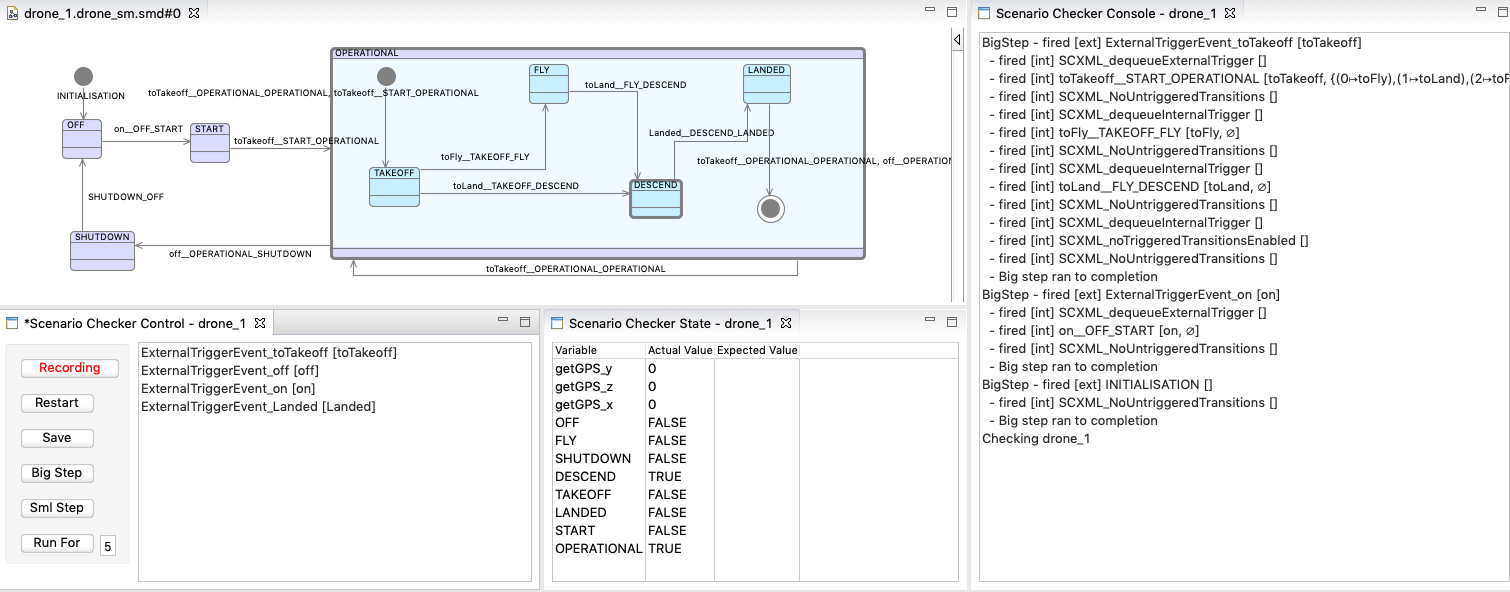
\includegraphics[width=0.90\textwidth, trim=30 50 60 0]{figures/scenarioChecker_recording_drone1.png}
	\caption{Using Scenario Checker to validate behaviour of refinement 1- recording}
	\label{fig:scenarioCheckerRecordingDrone1}
\end{figure}

Figure~\ref{fig:scenarioCheckerRecordingDrone1} shows a scenario being recorded.
The main (top-left) editing view shows the state-machine being animated; the model is currently in the |DESCEND| state.
The bottom left view is the scenario checker control panel where external events can be fired to start a run to completion.
In our model, only the external-trigger-raising events (representing the environment) are enabled.
The main button to be used is the \emph{Big Step} button which fires the selected external event and then automatically fires internal events until non are enabled.
The right hand view shows the scenario checker console, listing each big step and its run to completion in terms of internal events.
The bottom centre view shows the state of the system at the end of the last run.

\begin{figure}[!th]
	\centering
	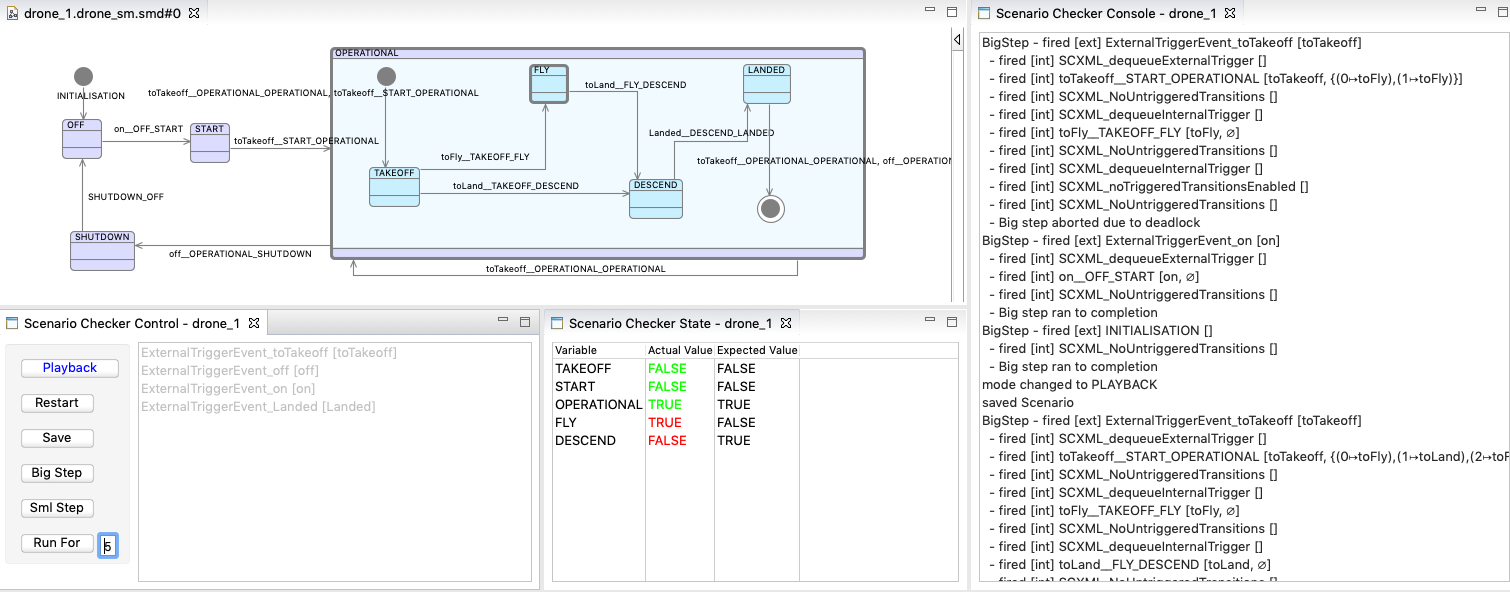
\includegraphics[width=0.90\textwidth, trim=30 50 60 0]{figures/scenarioChecker_playback_drone1.png}
	\caption{Using Scenario Checker to validate behaviour of refinement 1 - playback }
	\label{fig:scenarioCheckerPlaybackDrone1}
\end{figure}

Figure~\ref{fig:scenarioCheckerPlaybackDrone1} shows the recorded scenario being played back.
In the control panel, external events are greyed out as they are being selected from the recording each time the \emph{Big Step} button is pressed. 
The state view shows a discrepancy from when the scenario was recorded, and the state-machine is in the |FLY| state instead of the |DESCEND| state.
Comparing the history in the console panels reveals that cause: an internal trigger, |toLand|, was non-deterministically raised during recording but not during playback.
This is because the model allows for future raising of internal triggers in later refinements.

\begin{figure}[!th]
\centering
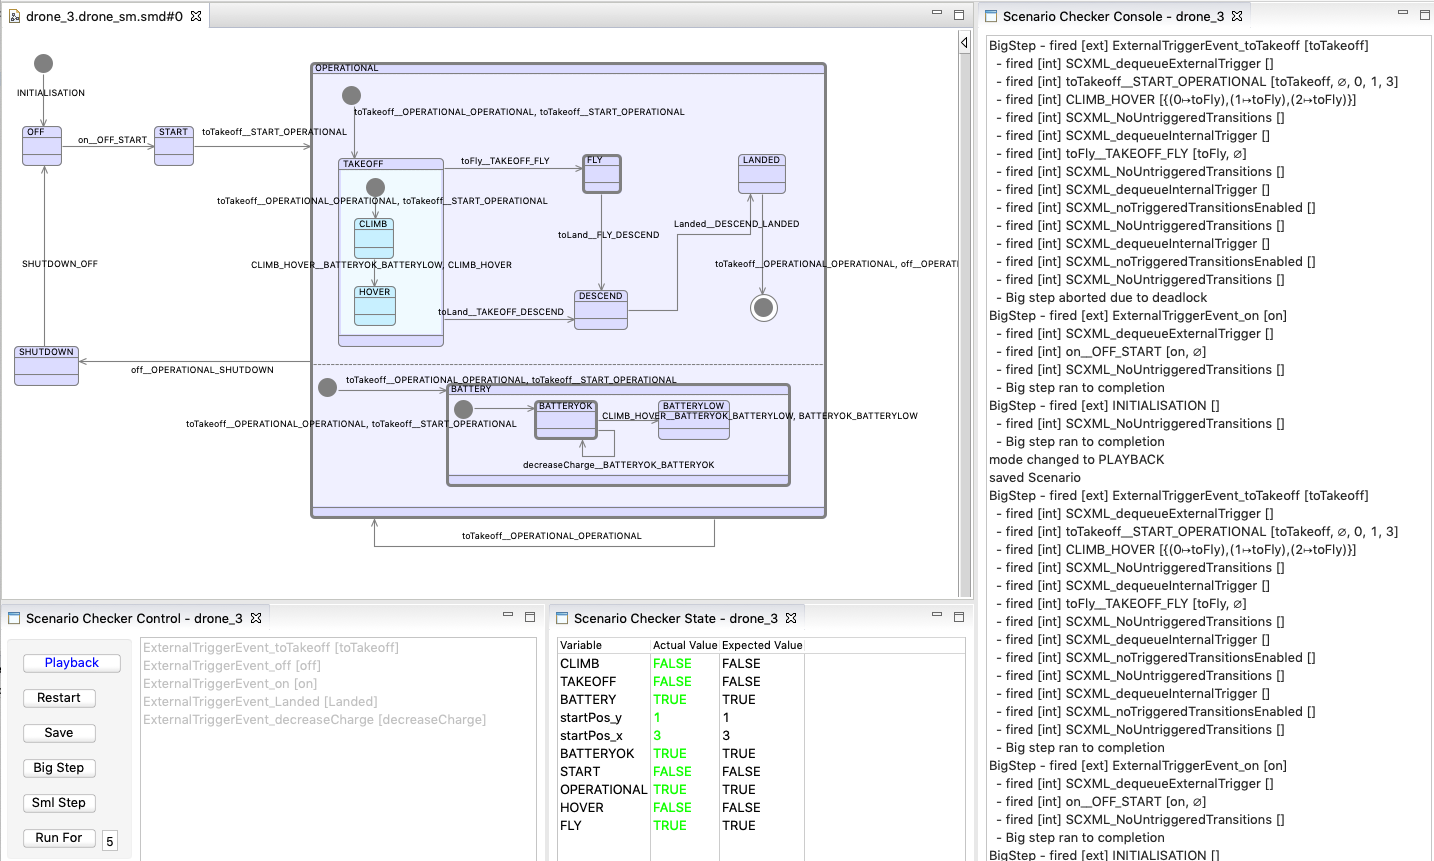
\includegraphics[width=0.90\textwidth, trim=30 50 60 0]{figures/scenarioChecker_playback_drone3.png}
\caption{Using Scenario Checker to validate behaviour of refinement 3 - playback}
\label{fig:scenarioCheckerPlaybackDrone3}
\end{figure}

Figure~\ref{fig:scenarioCheckerPlaybackDrone3} shows the scenario being played back at a later refinement where the raising of the |toFly| and |toLand| internal triggers has been defined. 
While the scenario checker allows us to animate that the main expected run to completion behaviour is possible, recall that, unless the transitions have all been finalised (i.e. no further refinement is permitted),  other behaviours are possible due to the non-deterministic completion incorporated in case transition guards are later strengthened. 
 

%%% Local Variables:
%%% mode: latex
%%% TeX-master: "../main"
%%% End:
